\section{Apache Spark}\label{sec:definition}
\par In this section we have a briefly insight of Spark architeture and we will know about running processes of Spark.
\par  Apache Spark \cite{apachespark} is the most popular open-source big data platforms in the world, which introduces the concept of resilient distributed datasets (RDDs) \cite{apachespark} to enable fast processing of large volume of data leveraging distributed memory. In memory data operation mechanism makes it well-suited for iterative applications such as iterative machine learning and graph algorithms. It need not swap data between harddisk and memory when it is running.
\par The Architecture of Spark is shown in Figure 1 as follows.
\begin{figure}[h]
	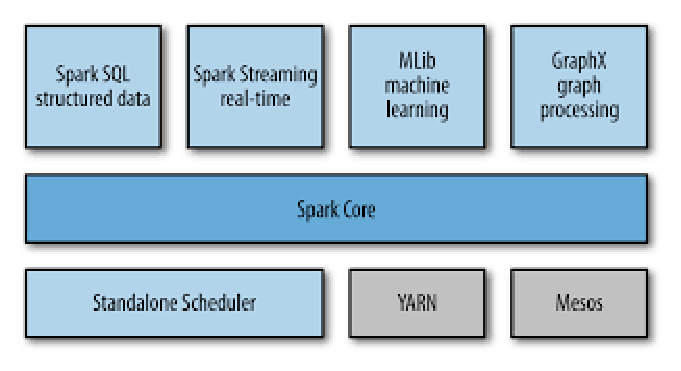
\includegraphics[width=8cm]{1.eps}
	\caption{Architecture of Apache Spark.}\label{fig:ArchitectureSpark}
\end{figure}
\par The main abstraction in Spark is resilient distributed dataset (RDD), which represents a read-only collection of objects distributed across a set of machines. Users can explicitly cache an RDD in memory across machines and reuse it in multiple MapReduce-like parallel operations. RDDs achieve fault tolerance through a notion of lineage: if a partition of an RDD is lost, the RDD has enough information about how it was derived from other RDDs to be able to rebuild just that partition. Although RDDs are not a general shared memory abstraction, they represent a sweet-spot between expressivity on the one hand and scalability and reliability on the other hand, and we have found them wellsuited for a variety of applications. 

\par Now we will show a typical deployment model of spark clusters (Standalone mode); A Spark cluster typically has multiple processes, each running in its own JVM, and a Spark cluster has a master node and multiple worker nodes, which are equivalent to Hadoop's master and slave nodes. The master node has a master daemon process, which manages all the worker nodes. The master daemon allocates resources across applications. The worker node has a worker daemon process, which is responsible for communicating with the master node and managing local executors. The worker also monitors the liveness and resource consumption of the executors. Each application has one driver and multiple executors. The tasks within the same executor belong to the same application. The driver is the process running the main function of the application and creating the SparkContext.
\par The following Figure \ref{fig:RunningSpark} describes the most significant processes.
\begin{figure}
	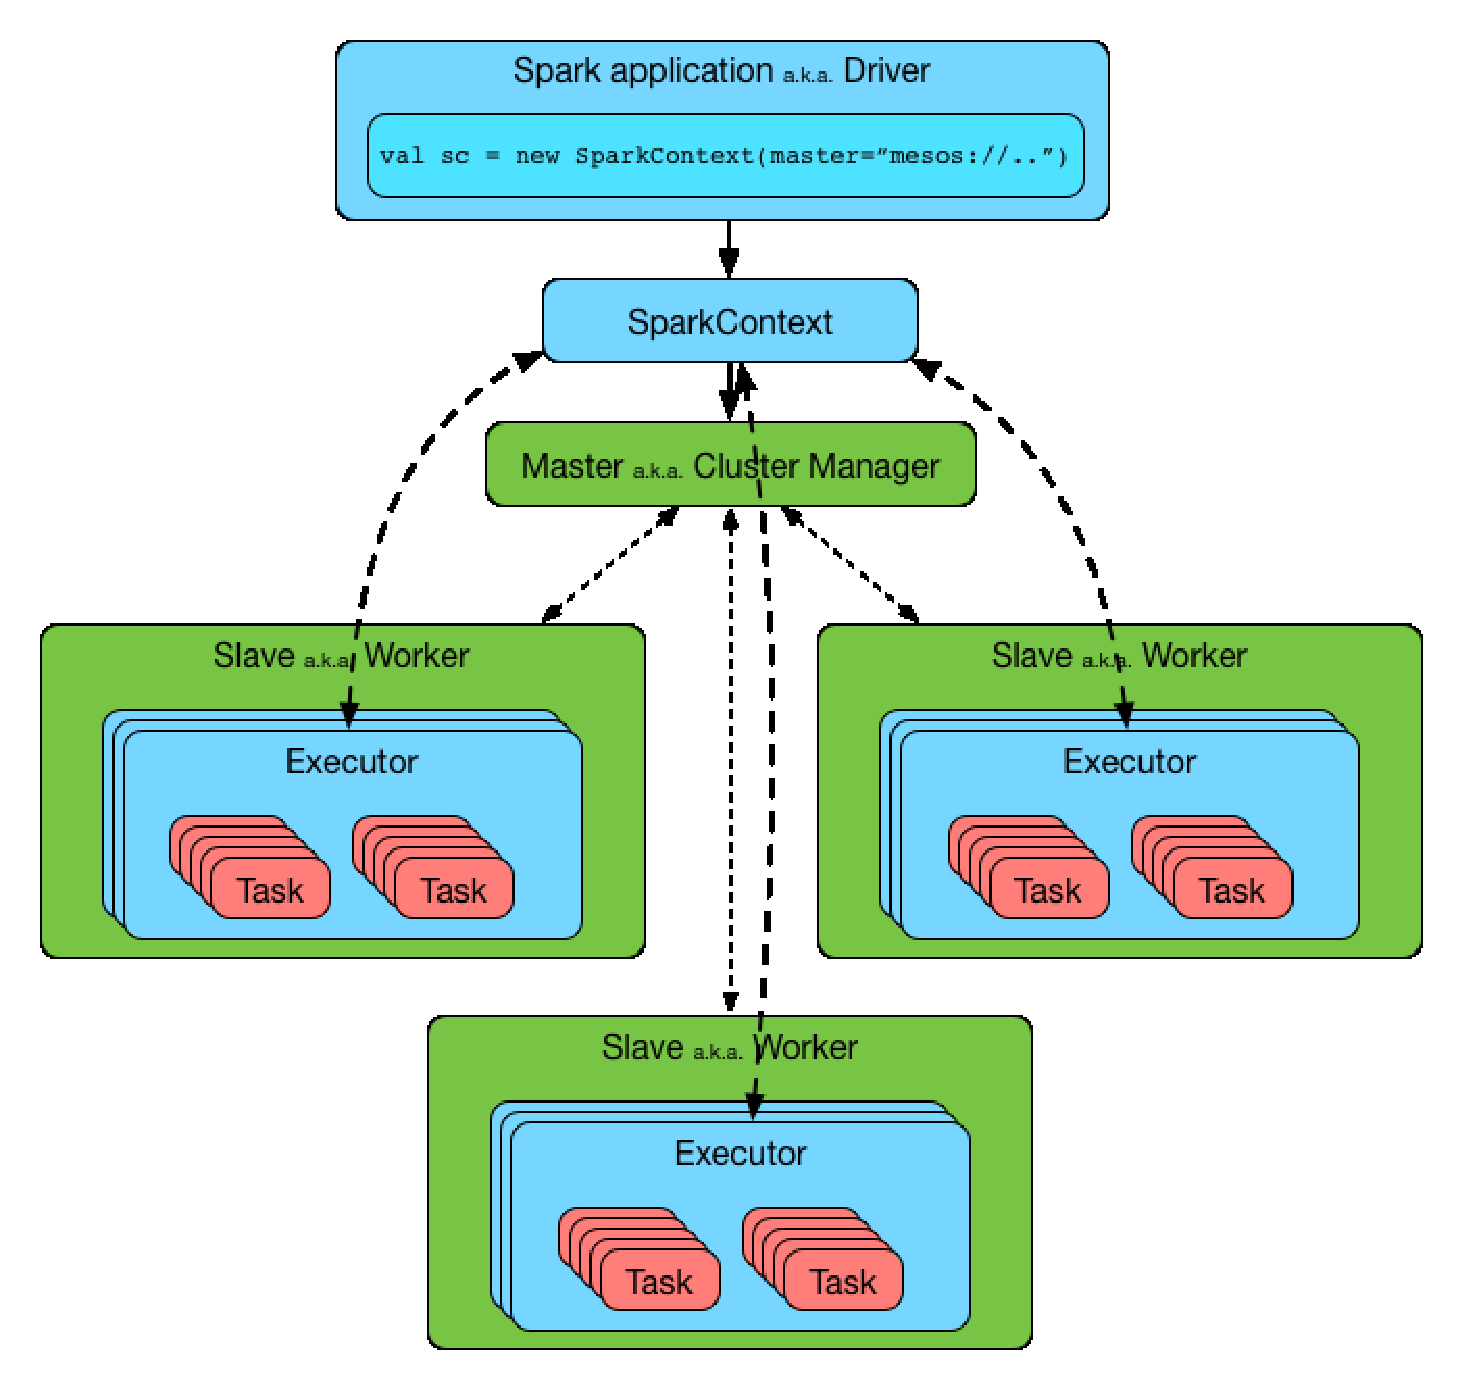
\includegraphics[width=8cm]{4.eps}
	\caption{Running Processes of Spark}\label{fig:RunningSpark}
\end{figure}

\par Because of the in-memory nature of most Spark computations, Spark programs can be bottlenecked by any resource in the cluster: CPU, network bandwidth, or memory. Most often, if the data fits in memory, the bottleneck is network bandwidth, but sometimes, you also need to do some tuning, such as storing RDDs in serialized form, to decrease memory usage. 

\par Fianlly we observe that Apache Spark tunning configuration is very complex, running process is very flexible by users different setting. Moreover we can also sample the parameters by system internal insight. Next we will look at the design of the Hummingbird.

